\documentclass[10pt]{article}

%%%%%%%% PREÁMBULO %%%%%%%%%%%%
\title{Plantilla para reportes Seminario de Tesis I}
\usepackage[spanish]{babel} %Indica que escribiermos en español
\usepackage[utf8]{inputenc} %Indica qué codificación se está usando ISO-8859-1(latin1)  o utf8  
\usepackage{amsmath} % Comandos extras para matemáticas (cajas para ecuaciones,
% etc)
\usepackage{amssymb} % Simbolos matematicos (por lo tanto)
\usepackage{graphicx} % Incluir imágenes en LaTeX
\usepackage{color} % Para colorear texto
\usepackage{subfigure} % subfiguras
\usepackage{float} %Podemos usar el especificador [H] en las figuras para que se
% queden donde queramos
\usepackage{capt-of} % Permite usar etiquetas fuera de elementos flotantes
% (etiquetas de figuras)
\usepackage{sidecap} % Para poner el texto de las imágenes al lado
	\sidecaptionvpos{figure}{c} % Para que el texto se alinie al centro vertical
\usepackage{caption} % Para poder quitar numeracion de figuras
\usepackage{commath} % funcionalidades extras para diferenciales, integrales,
% etc (\od, \dif, etc)
\usepackage{cancel} % para cancelar expresiones (\cancelto{0}{x})
 
\usepackage{anysize} 					% Para personalizar el ancho de  los márgenes
\marginsize{2cm}{2cm}{1.0cm}{2.5cm} % Izquierda, derecha, arriba, abajo

\usepackage{setspace} % Para modificar el interlineado por parrafos en el texto.

\usepackage{appendix}
\renewcommand{\appendixname}{Apéndice}
\renewcommand{\appendixtocname}{Apéndice}
\renewcommand{\appendixpagename}{Apéndice} 

% Para que las referencias sean hipervínculos a las figuras o ecuaciones y
% aparezcan en color
\usepackage[colorlinks=true,plainpages=true,citecolor=blue,linkcolor=blue,urlcolor=blue]{hyperref}
%\usepackage{hyperref} 
% Para agregar encabezado y pie de página
\usepackage{fancyhdr} 
\pagestyle{fancy}
\fancyhf{}
\setlength{\headheight}{45pt}
\fancyhead[L]{
\includegraphics[scale=0.075]{Logo_Cinves.png}} %encabezado izquierda
\fancyhead[R]{\footnotesize Departamento de Robótica y Manufactura Avanzada}   % dereecha
\fancyfoot[R]{\footnotesize Manufactura II}  % Pie derecha
\fancyfoot[C]{\thepage}  % centro
\fancyfoot[L]{\footnotesize Maestría en Robótica y Man. Avanzada}  %izquierda
\renewcommand{\footrulewidth}{0.4pt}


\usepackage{listings} % Para usar código fuente
\definecolor{dkgreen}{rgb}{0,0.6,0} % Definimos colores para usar en el código
\definecolor{gray}{rgb}{0.5,0.5,0.5} 
% configuración para el lenguaje que queramos utilizar
\lstset{language=Matlab,
   keywords={break,case,catch,continue,else,elseif,end,for,function,
      global,if,otherwise,persistent,return,switch,try,while},
   basicstyle=\ttfamily,
   keywordstyle=\color{blue},
   commentstyle=\color{red},
   stringstyle=\color{dkgreen},
   numbers=left,
   numberstyle=\tiny\color{gray},
   stepnumber=1,
   numbersep=10pt,
   backgroundcolor=\color{white},
   tabsize=4,
   showspaces=false,
   showstringspaces=false}

\newcommand{\sen}{\operatorname{\sen}}	% Definimos el comando \sen para el seno en español

% Basada en la plantilla para reportes UPIITA de  Overleaf
%%%%%%%% TERMINA PREÁMBULO %%%%%%%%%%%%

\graphicspath{ {../imagenes/} } % Directorio raiz para las imagenes

%\title{Desarrollo de la teoría de la relatividad especial de Einstein}

\begin{document}

    %%%%%%%%%%%%%%%%%%%%%%%%%%%%%%%%%% PORTADA %%%%%%%%%%%%%%%%%%%%%%%%%%%%%%%%%%%%%%%%%%%%
\begin{center}
    \newcommand{\HRule}{\rule{\linewidth}{0.5mm}}
    \vspace*{0.5cm}

    \begin{spacing}{1.5}
        \textsc{\huge Centro de Investigación y de Estudios Avanzados del Instituto Politecnico Nacional}\\[0.15cm]
    \end{spacing}

    \begin{center}
        
\includegraphics[scale=0.35]{Logo_Cinves.png}
    \end{center}

    \begin{minipage}{0.9\textwidth}
        \begin{center}
            \textbf{\Large Manufactura II}\\
            \vspace*{0.5cm}
            \textsc{\LARGE Tarea 4 }
        \end{center}
    \end{minipage}\\[0.1cm]

 	\vspace*{1cm}

    \HRule \\[0.4cm]{\huge \bfseries ART-1}\\[0.4cm] % Titulo del reporte
    \HRule \\[1.5cm]

    \begin{minipage}{\textwidth}
        \begin{flushleft} \large
            % Aqui a continuación pongan los nombres de los integrantes
            \emph{\textbf{Autor}:}\\
            Luis Ángel Torres Martínez  (214520012)
        \end{flushleft}
    \end{minipage}

    \begin{minipage}{\textwidth}
        \vspace{-1cm}
        \begin{flushright} \large
            \emph{\textbf{Profesor(a)}:} \\
            Dr. Ismael López Juárez \\
        \end{flushright}
    \end{minipage}

    \vspace{3cm}
    
    Saltillo, Coahuila, México \\ % Lugar de redacción
    09 de Octubre de 2022\\ % Fecha de creación
    ultima edición: {\today} % Fecha de última modificación
\end{center}

    \newpage

    \tableofcontents

    \newpage

    %\section{Resumen}
    %En el presente trabajo se presentará y describirá de maner breve un mapa mental en donde se plasman aquellas
actividades en las cuales invierto mi tiempo.

    %\section{Introducción}
    %Una red neuronal esta compuesta por varios perceptrones y su salida sigue las mismas reglas que el
perceptrón, es decir, se realiza la suma ponderada de las entradas y después esta se hace pasar por una
función de activación. Esta operación se realiza de manera recursiva de manera que, la entrada de la capa
subsecuente corresponde a la salida de la capa actual. De esta manera, mediante la interconexión de
varios perceptrones es posible generar funciones no lineales.\\
La manera en que aprenden las redes neuronales es mediante la minimización de una función de costo, como
puede ser el error cuadrático medio (MSE), ReLu, entre otras. Una vez que se tiene la función de costo,
se utiliza la técnica del descenso del gradiente para minimizar esta función y mediante esta técnica la
red neuronal ``aprende''. Como técnica utilizada para obtener el gradiente se utiliza el algoritmo de
\textbf{backpropagation}.

    %\section{Desarrollo}
    %Se implemento una red neuronal que consiste en 1 capa de entrada y 1 capa de salida, cada capa contiene
1 sola neurona, el vector de entrada es de tamaño 2 y la red tiene una topología \textit{fully connected}.
\begin{figure}[H]
    \centering
    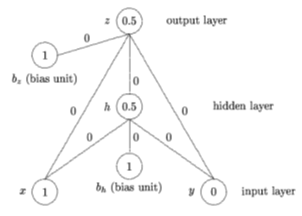
\includegraphics{Net_Topology.png}
    \caption{Topología de la red}
    \label{fig:NetTopology}
\end{figure}
Se realizó el entrenamiento de las 3 redes neuronales con diferentes ordenes dados en el ``dataset'' de
entrenamiento, diferentes tasas de aprendizaje y diferentes tipos de batch.\\[0.5cm]
\textbf{Tasas de aprendizaje}:\\
0.1 - 0.5 - 1 - 2 - 3 - 4 - 5\\[0.5cm]
\textbf{Tamaños de lote}:\\
1 - 2 - 4\\[0.5cm]

El tamaño del batch 1 significa entrenamiento en linea, el batch de 4 es el entrenamiento por lote y el
batch 2 es entrenamiento de medio lote.

\newpage
\subsection{Resultados}
%%%%%%%%%%%%%%%%%%%%%%%%%%%%%%%%%%%%%%%%%%%%%%%%%%%%%%%%%%%%%%%%%%%%%%%%%%%%%%%%%%%%%%%%%%%%%%%%%%%%%%
%%%%%%%%%%%%%%%%%%                            Orden 1                             %%%%%%%%%%%%%%%%%%%%
%%%%%%%%%%%%%%%%%%%%%%%%%%%%%%%%%%%%%%%%%%%%%%%%%%%%%%%%%%%%%%%%%%%%%%%%%%%%%%%%%%%%%%%%%%%%%%%%%%%%%%
\subsubsection{Orden 1}
\begin{table}[H]
    \centering
    \begin{tabular}{|ll|l|l|l|}
    \hline
    \multicolumn{2}{|c|}{\textbf{In}} & \multicolumn{1}{c|}{\textbf{And}} & \multicolumn{1}{c|}{\textbf{Or}} & \multicolumn{1}{c|}{\textbf{Xor}} \\ \hline
    \multicolumn{1}{|l|}{0}    & 0    & 0                                 & 0                                & 0                                 \\ \hline
    \multicolumn{1}{|l|}{0}    & 1    & 0                                 & 1                                & 1                                 \\ \hline
    \multicolumn{1}{|l|}{1}    & 0    & 0                                 & 1                                & 1                                 \\ \hline
    \multicolumn{1}{|l|}{1}    & 1    & 1                                 & 1                                & 0                                 \\ \hline
    \end{tabular}
\end{table}
El entrenamiento de la red se realizó con los siguientes resultados:
\begin{table}[H]
    \begin{tabular}{|l|lllllllll|}
    \hline
    \multicolumn{1}{|c|}{\multirow{3}{*}{\textbf{$\eta$}}} & \multicolumn{9}{c|}{\textbf{Epocas}}                                                                                                                                                                                                                                                                      \\ \cline{2-10} 
    \multicolumn{1}{|c|}{}                                 & \multicolumn{3}{l|}{\textbf{En línea}}                                                                   & \multicolumn{3}{l|}{\textbf{Batch (4)}}                                                                  & \multicolumn{3}{l|}{\textbf{Batch (2)}}                                             \\ \cline{2-10} 
    \multicolumn{1}{|c|}{}                                 & \multicolumn{1}{l|}{\textbf{And}} & \multicolumn{1}{l|}{\textbf{Or}} & \multicolumn{1}{l|}{\textbf{Xor}} & \multicolumn{1}{l|}{\textbf{And}} & \multicolumn{1}{l|}{\textbf{Or}} & \multicolumn{1}{l|}{\textbf{Xor}} & \multicolumn{1}{l|}{\textbf{And}} & \multicolumn{1}{l|}{\textbf{Or}} & \textbf{Xor} \\ \hline
    0.1                                                    & \multicolumn{1}{l|}{13253}        & \multicolumn{1}{l|}{11276}       & \multicolumn{1}{l|}{22990}        & \multicolumn{1}{l|}{25183}        & \multicolumn{1}{l|}{36909}       & \multicolumn{1}{l|}{más de 50000} & \multicolumn{1}{l|}{14884}        & \multicolumn{1}{l|}{22248}       & más de 50000 \\ \hline
    0.5                                                    & \multicolumn{1}{l|}{1342}         & \multicolumn{1}{l|}{1666}        & \multicolumn{1}{l|}{6592}         & \multicolumn{1}{l|}{5386}         & \multicolumn{1}{l|}{6992}        & \multicolumn{1}{l|}{19240}        & \multicolumn{1}{l|}{5330}         & \multicolumn{1}{l|}{4383}        & 10893        \\ \hline
    1                                                      & \multicolumn{1}{l|}{672}          & \multicolumn{1}{l|}{1141}        & \multicolumn{1}{l|}{3332}         & \multicolumn{1}{l|}{5313}         & \multicolumn{1}{l|}{4403}        & \multicolumn{1}{l|}{10176}        & \multicolumn{1}{l|}{1460}         & \multicolumn{1}{l|}{2308}        & 4610         \\ \hline
    2                                                      & \multicolumn{1}{l|}{638}          & \multicolumn{1}{l|}{465}         & \multicolumn{1}{l|}{1518}         & \multicolumn{1}{l|}{2648}         & \multicolumn{1}{l|}{1896}        & \multicolumn{1}{l|}{4608}         & \multicolumn{1}{l|}{638}          & \multicolumn{1}{l|}{944}         & 4762         \\ \hline
    3                                                      & \multicolumn{1}{l|}{382}          & \multicolumn{1}{l|}{386}         & \multicolumn{1}{l|}{más de 50000} & \multicolumn{1}{l|}{905}          & \multicolumn{1}{l|}{1486}        & \multicolumn{1}{l|}{5237}         & \multicolumn{1}{l|}{875}          & \multicolumn{1}{l|}{613}         & 1560         \\ \hline
    4                                                      & \multicolumn{1}{l|}{152}          & \multicolumn{1}{l|}{283}         & \multicolumn{1}{l|}{más de 50000} & \multicolumn{1}{l|}{1327}         & \multicolumn{1}{l|}{1101}        & \multicolumn{1}{l|}{2520}         & \multicolumn{1}{l|}{325}          & \multicolumn{1}{l|}{552}         & 1678         \\ \hline
    5                                                      & \multicolumn{1}{l|}{241}          & \multicolumn{1}{l|}{226}         & \multicolumn{1}{l|}{más de 50000} & \multicolumn{1}{l|}{1063}         & \multicolumn{1}{l|}{884}         & \multicolumn{1}{l|}{1838}         & \multicolumn{1}{l|}{297}          & \multicolumn{1}{l|}{398}         & 942          \\ \hline
    \end{tabular}
\end{table}

\begin{figure}[H]
    \centering
    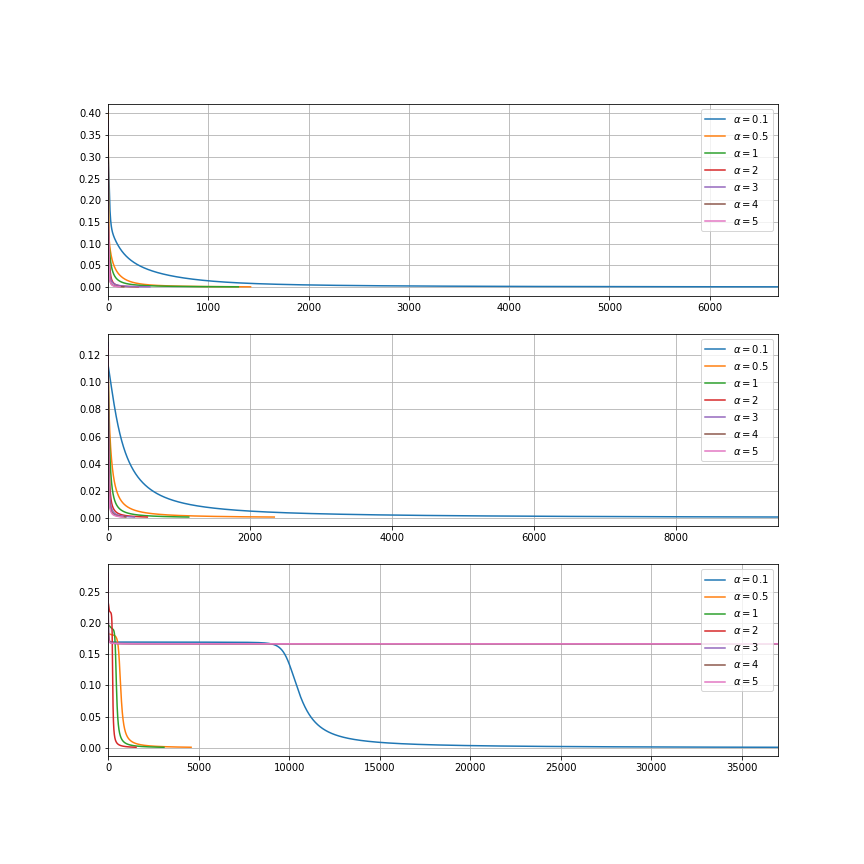
\includegraphics[width=17cm,height=12cm]{Training Batch 1 Orden 1.png}
    \caption{Entrenamiento de las redes con batch 1 (De arriba a abajo: And,Or,Xor)}
    \label{fig:TrainBatch1_Order1}
\end{figure}
\begin{figure}[H]
    \centering
    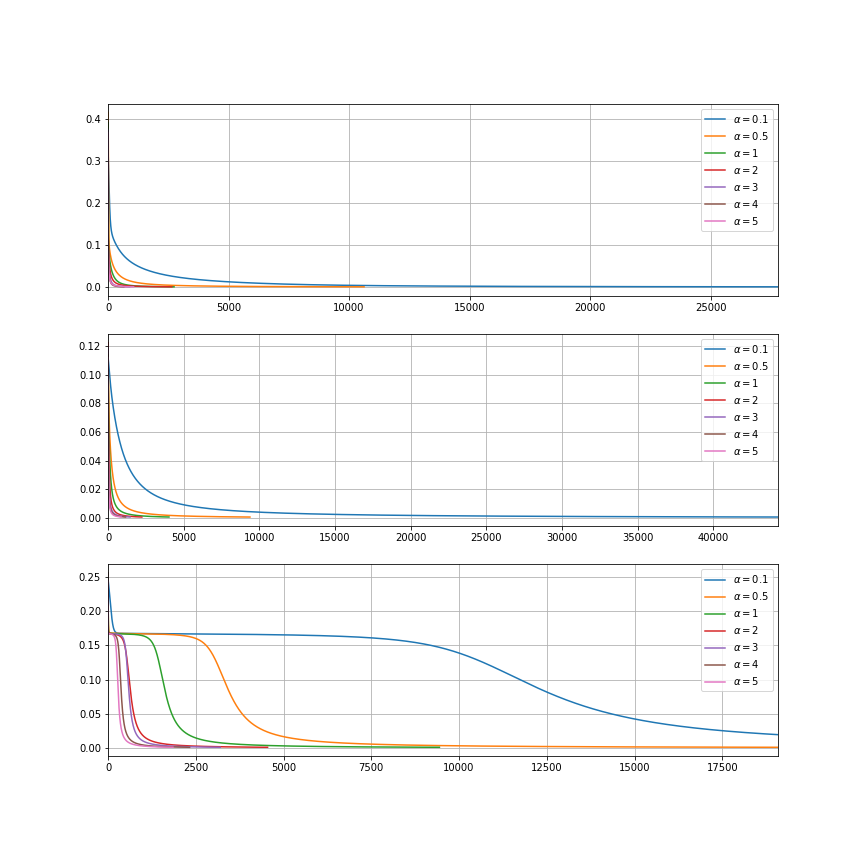
\includegraphics[width=17cm,height=20cm]{Training Batch 4 Orden 1.png}
    \caption{Entrenamiento de las redes con batch 4 (De arriba a abajo: And,Or,Xor)}
    \label{fig:TrainBatch4_Order1}
\end{figure}
\begin{figure}[H]
    \centering
    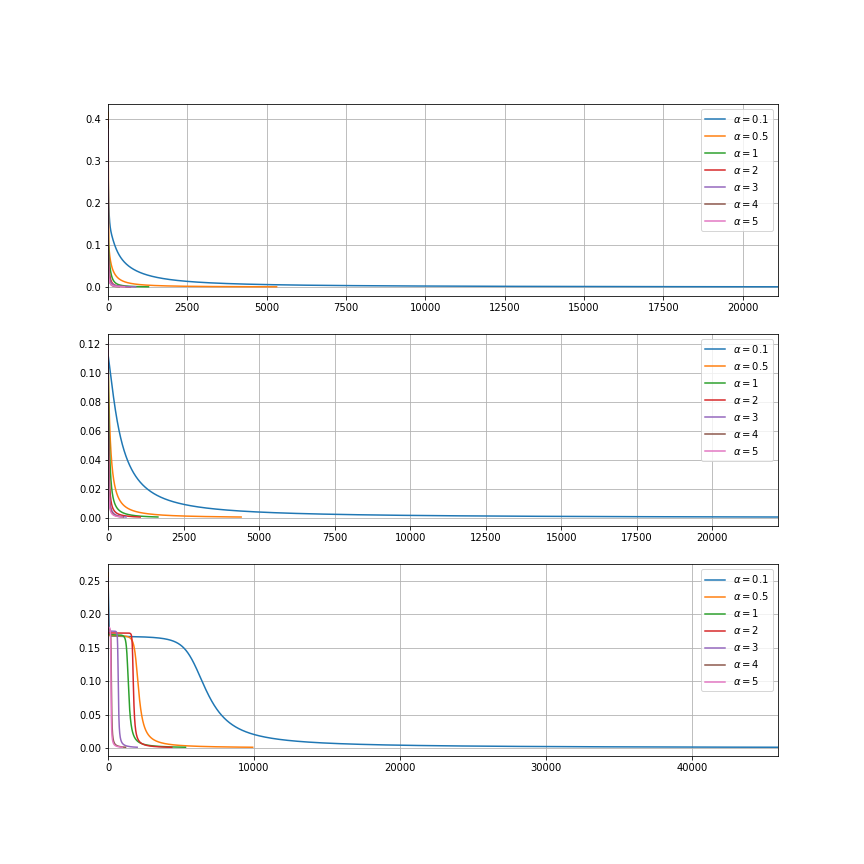
\includegraphics[width=17cm,height=20cm]{Training Batch 2 Orden 1.png}
    \caption{Entrenamiento de las redes con batch 2 (De arriba a abajo: And,Or,Xor)}
    \label{fig:TrainBatch2_Order1}
\end{figure}

%%%%%%%%%%%%%%%%%%%%%%%%%%%%%%%%%%%%%%%%%%%%%%%%%%%%%%%%%%%%%%%%%%%%%%%%%%%%%%%%%%%%%%%%%%%%%%%%%%%%%%
%%%%%%%%%%%%%%%%%%                            Orden 2                             %%%%%%%%%%%%%%%%%%%%
%%%%%%%%%%%%%%%%%%%%%%%%%%%%%%%%%%%%%%%%%%%%%%%%%%%%%%%%%%%%%%%%%%%%%%%%%%%%%%%%%%%%%%%%%%%%%%%%%%%%%%

\subsubsection{Orden 2}
\begin{table}[H]
    \centering
    \begin{tabular}{|ll|l|l|l|}
    \hline
    \multicolumn{2}{|c|}{\textbf{In}} & \multicolumn{1}{c|}{\textbf{And}} & \multicolumn{1}{c|}{\textbf{Or}} & \multicolumn{1}{c|}{\textbf{Xor}} \\ \hline
    \multicolumn{1}{|l|}{1}    & 1    & 1                                 & 1                                & 0                                 \\ \hline
    \multicolumn{1}{|l|}{1}    & 0    & 0                                 & 1                                & 1                                 \\ \hline
    \multicolumn{1}{|l|}{0}    & 1    & 0                                 & 1                                & 1                                 \\ \hline
    \multicolumn{1}{|l|}{0}    & 0    & 0                                 & 0                                & 0                                 \\ \hline
    \end{tabular}
\end{table}
El entrenamiento de la red se realizó con los siguientes resultados:
\begin{table}[H]
    \begin{tabular}{|l|lllllllll|}
    \hline
    \multicolumn{1}{|c|}{\multirow{3}{*}{\textbf{$\eta$}}} & \multicolumn{9}{c|}{\textbf{Epocas}}                                                                                                                                                                                                                                                                      \\ \cline{2-10} 
    \multicolumn{1}{|c|}{}                                 & \multicolumn{3}{l|}{\textbf{En línea}}                                                                   & \multicolumn{3}{l|}{\textbf{Batch (4)}}                                                                  & \multicolumn{3}{l|}{\textbf{Batch (2)}}                                             \\ \cline{2-10} 
    \multicolumn{1}{|c|}{}                                 & \multicolumn{1}{l|}{\textbf{And}} & \multicolumn{1}{l|}{\textbf{Or}} & \multicolumn{1}{l|}{\textbf{Xor}} & \multicolumn{1}{l|}{\textbf{And}} & \multicolumn{1}{l|}{\textbf{Or}} & \multicolumn{1}{l|}{\textbf{Xor}} & \multicolumn{1}{l|}{\textbf{And}} & \multicolumn{1}{l|}{\textbf{Or}} & \textbf{Xor} \\ \hline
    0.1                                                    & \multicolumn{1}{l|}{6620}         & \multicolumn{1}{l|}{10204}       & \multicolumn{1}{l|}{24852}        & \multicolumn{1}{l|}{45865}        & \multicolumn{1}{l|}{46051}       & \multicolumn{1}{l|}{más de 50000} & \multicolumn{1}{l|}{26595}        & \multicolumn{1}{l|}{22632}       & más de 50000 \\ \hline
    0.5                                                    & \multicolumn{1}{l|}{1433}         & \multicolumn{1}{l|}{2249}        & \multicolumn{1}{l|}{6338}         & \multicolumn{1}{l|}{5284}         & \multicolumn{1}{l|}{8779}        & \multicolumn{1}{l|}{más de 50000} & \multicolumn{1}{l|}{3123}         & \multicolumn{1}{l|}{4169}        & 17154        \\ \hline
    1                                                      & \multicolumn{1}{l|}{1307}         & \multicolumn{1}{l|}{1160}        & \multicolumn{1}{l|}{2764}         & \multicolumn{1}{l|}{5304}         & \multicolumn{1}{l|}{4550}        & \multicolumn{1}{l|}{9750}         & \multicolumn{1}{l|}{2644}         & \multicolumn{1}{l|}{2232}        & 4943         \\ \hline
    2                                                      & \multicolumn{1}{l|}{312}          & \multicolumn{1}{l|}{523}         & \multicolumn{1}{l|}{1718}         & \multicolumn{1}{l|}{1354}         & \multicolumn{1}{l|}{2177}        & \multicolumn{1}{l|}{5330}         & \multicolumn{1}{l|}{1245}         & \multicolumn{1}{l|}{1127}        & 7881         \\ \hline
    3                                                      & \multicolumn{1}{l|}{216}          & \multicolumn{1}{l|}{317}         & \multicolumn{1}{l|}{851}          & \multicolumn{1}{l|}{1770}         & \multicolumn{1}{l|}{1523}        & \multicolumn{1}{l|}{2948}         & \multicolumn{1}{l|}{879}          & \multicolumn{1}{l|}{688}         & 1694         \\ \hline
    4                                                      & \multicolumn{1}{l|}{170}          & \multicolumn{1}{l|}{289}         & \multicolumn{1}{l|}{más de 50000} & \multicolumn{1}{l|}{1325}         & \multicolumn{1}{l|}{974}         & \multicolumn{1}{l|}{más de 50000} & \multicolumn{1}{l|}{318}          & \multicolumn{1}{l|}{540}         & 1272         \\ \hline
    5                                                      & \multicolumn{1}{l|}{134}          & \multicolumn{1}{l|}{194}         & \multicolumn{1}{l|}{más de 50000} & \multicolumn{1}{l|}{1062}         & \multicolumn{1}{l|}{824}         & \multicolumn{1}{l|}{1782}         & \multicolumn{1}{l|}{364}          & \multicolumn{1}{l|}{415}         & más de 50000 \\ \hline
    \end{tabular}
\end{table}
\begin{figure}[H]
    \centering
    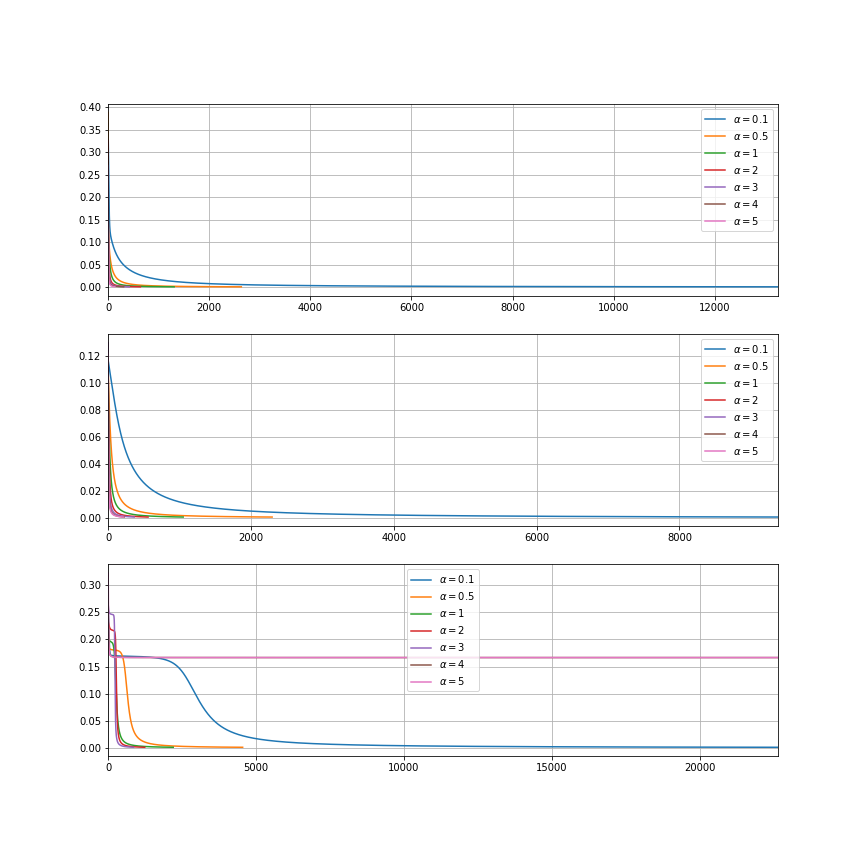
\includegraphics[width=17cm,height=13cm]{Training Batch 1 Orden 2.png}
    \caption{Entrenamiento de las redes con batch 1 (De arriba a abajo: And,Or,Xor)}
    \label{fig:TrainBatch1_Order2}
\end{figure}
\begin{figure}[H]
    \centering
    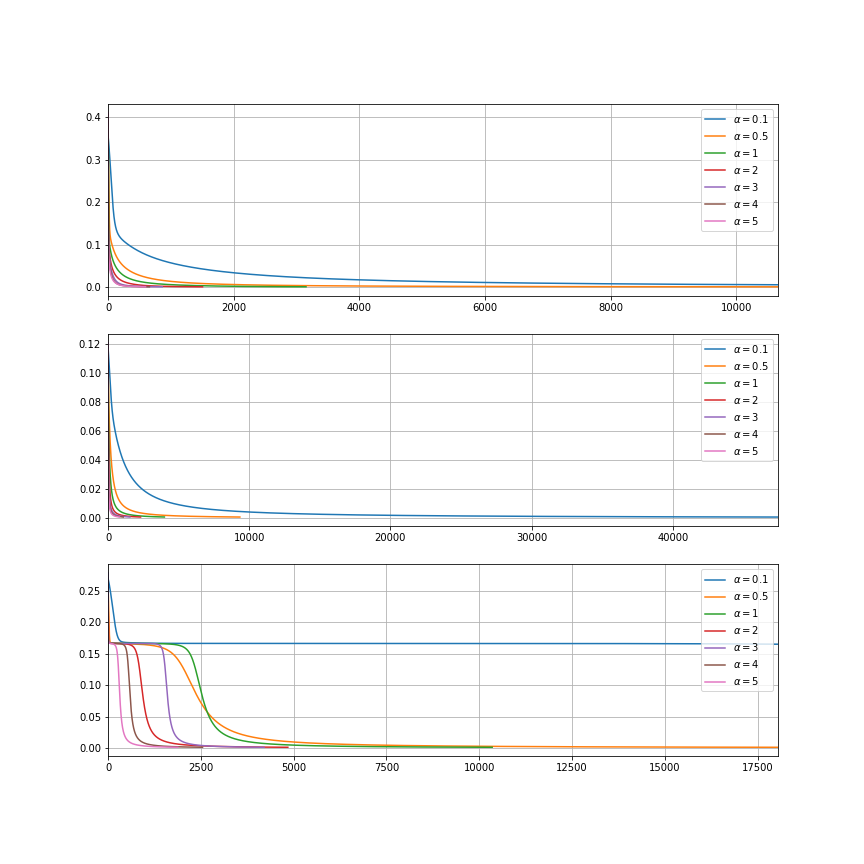
\includegraphics[width=17cm,height=20cm]{Training Batch 4 Orden 2.png}
    \caption{Entrenamiento de las redes con batch 4 (De arriba a abajo: And,Or,Xor)}
    \label{fig:TrainBatch4_Order2}
\end{figure}
\begin{figure}[H]
    \centering
    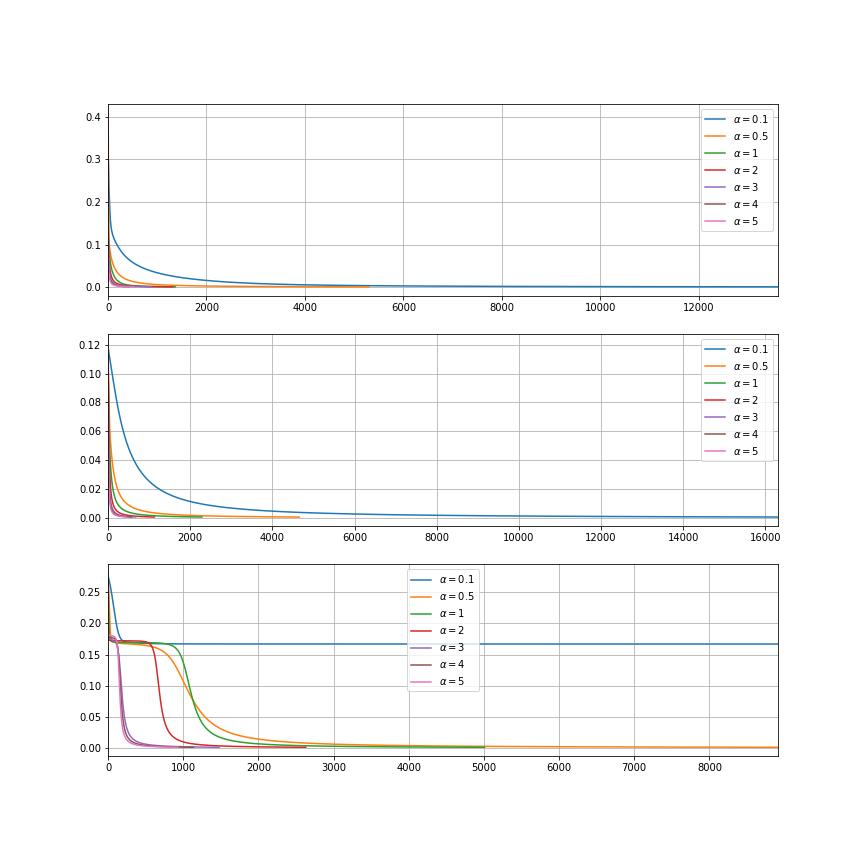
\includegraphics[width=17cm,height=20cm]{Training Batch 2 Orden 2.png}
    \caption{Entrenamiento de las redes con batch 2 (De arriba a abajo: And,Or,Xor)}
    \label{fig:TrainBatch2_Order2}
\end{figure}

%%%%%%%%%%%%%%%%%%%%%%%%%%%%%%%%%%%%%%%%%%%%%%%%%%%%%%%%%%%%%%%%%%%%%%%%%%%%%%%%%%%%%%%%%%%%%%%%%%%%%%
%%%%%%%%%%%%%%%%%%                            Orden 3                             %%%%%%%%%%%%%%%%%%%%
%%%%%%%%%%%%%%%%%%%%%%%%%%%%%%%%%%%%%%%%%%%%%%%%%%%%%%%%%%%%%%%%%%%%%%%%%%%%%%%%%%%%%%%%%%%%%%%%%%%%%%

\subsubsection{Orden 3}
\begin{table}[H]
    \centering
    \begin{tabular}{|ll|l|l|l|}
    \hline
    \multicolumn{2}{|c|}{\textbf{In}} & \multicolumn{1}{c|}{\textbf{And}} & \multicolumn{1}{c|}{\textbf{Or}} & \multicolumn{1}{c|}{\textbf{Xor}} \\ \hline
    \multicolumn{1}{|l|}{0}    & 0    & 0                                 & 0                                & 0                                 \\ \hline
    \multicolumn{1}{|l|}{1}    & 1    & 1                                 & 1                                & 0                                 \\ \hline
    \multicolumn{1}{|l|}{0}    & 1    & 0                                 & 1                                & 1                                 \\ \hline
    \multicolumn{1}{|l|}{1}    & 0    & 0                                 & 1                                & 1                                 \\ \hline
    \end{tabular}
\end{table}
El entrenamiento de la red se realizó con los siguientes resultados:
\begin{table}[H]
    \begin{tabular}{|l|lllllllll|}
    \hline
    \multicolumn{1}{|c|}{\multirow{3}{*}{\textbf{$\eta$}}} & \multicolumn{9}{c|}{\textbf{Epocas}}                                                                                                                                                                                                                                                                      \\ \cline{2-10} 
    \multicolumn{1}{|c|}{}                                 & \multicolumn{3}{l|}{\textbf{En línea}}                                                                   & \multicolumn{3}{l|}{\textbf{Batch (4)}}                                                                  & \multicolumn{3}{l|}{\textbf{Batch (2)}}                                             \\ \cline{2-10} 
    \multicolumn{1}{|c|}{}                                 & \multicolumn{1}{l|}{\textbf{And}} & \multicolumn{1}{l|}{\textbf{Or}} & \multicolumn{1}{l|}{\textbf{Xor}} & \multicolumn{1}{l|}{\textbf{And}} & \multicolumn{1}{l|}{\textbf{Or}} & \multicolumn{1}{l|}{\textbf{Xor}} & \multicolumn{1}{l|}{\textbf{And}} & \multicolumn{1}{l|}{\textbf{Or}} & \textbf{Xor} \\ \hline
    0.1                                                    & \multicolumn{1}{l|}{13302}        & \multicolumn{1}{l|}{10281}       & \multicolumn{1}{l|}{37423}        & \multicolumn{1}{l|}{27350}        & \multicolumn{1}{l|}{45932}       & \multicolumn{1}{l|}{más de 50000} & \multicolumn{1}{l|}{26483}        & \multicolumn{1}{l|}{22010}       & más de 50000 \\ \hline
    0.5                                                    & \multicolumn{1}{l|}{1416}         & \multicolumn{1}{l|}{2176}        & \multicolumn{1}{l|}{4403}         & \multicolumn{1}{l|}{10607}        & \multicolumn{1}{l|}{7013}        & \multicolumn{1}{l|}{23004}        & \multicolumn{1}{l|}{5288}         & \multicolumn{1}{l|}{3889}        & 21725        \\ \hline
    1                                                      & \multicolumn{1}{l|}{727}          & \multicolumn{1}{l|}{1117}        & \multicolumn{1}{l|}{2647}         & \multicolumn{1}{l|}{5298}         & \multicolumn{1}{l|}{4066}        & \multicolumn{1}{l|}{9516}         & \multicolumn{1}{l|}{1332}         & \multicolumn{1}{l|}{2243}        & 7101         \\ \hline
    2                                                      & \multicolumn{1}{l|}{335}          & \multicolumn{1}{l|}{531}         & \multicolumn{1}{l|}{1262}         & \multicolumn{1}{l|}{2659}         & \multicolumn{1}{l|}{2238}        & \multicolumn{1}{l|}{más de 50000} & \multicolumn{1}{l|}{1302}         & \multicolumn{1}{l|}{1119}        & 2207         \\ \hline
    3                                                      & \multicolumn{1}{l|}{217}          & \multicolumn{1}{l|}{353}         & \multicolumn{1}{l|}{801}          & \multicolumn{1}{l|}{962}          & \multicolumn{1}{l|}{1545}        & \multicolumn{1}{l|}{más de 50000} & \multicolumn{1}{l|}{860}          & \multicolumn{1}{l|}{767}         & 2055         \\ \hline
    4                                                      & \multicolumn{1}{l|}{309}          & \multicolumn{1}{l|}{250}         & \multicolumn{1}{l|}{más de 50000} & \multicolumn{1}{l|}{1297}         & \multicolumn{1}{l|}{909}         & \multicolumn{1}{l|}{2321}         & \multicolumn{1}{l|}{328}          & \multicolumn{1}{l|}{432}         & 1654         \\ \hline
    5                                                      & \multicolumn{1}{l|}{244}          & \multicolumn{1}{l|}{221}         & \multicolumn{1}{l|}{más de 50000} & \multicolumn{1}{l|}{652}          & \multicolumn{1}{l|}{872}         & \multicolumn{1}{l|}{1765}         & \multicolumn{1}{l|}{260}          & \multicolumn{1}{l|}{446}         & más de 50000 \\ \hline
    \end{tabular}
    \end{table}
\begin{figure}[H]
    \centering
    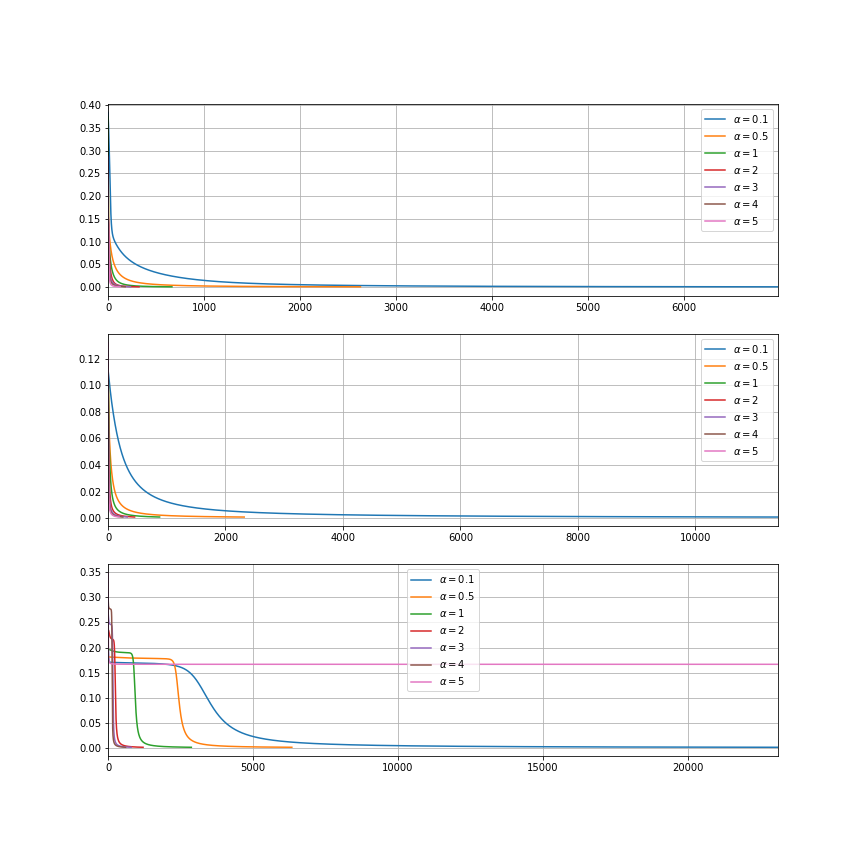
\includegraphics[width=17cm,height=13cm]{Training Batch 1 Orden 3.png}
    \caption{Entrenamiento de las redes con batch 1 (De arriba a abajo: And,Or,Xor)}
    \label{fig:TrainBatch1_Order3}
\end{figure}
\begin{figure}[H]
    \centering
    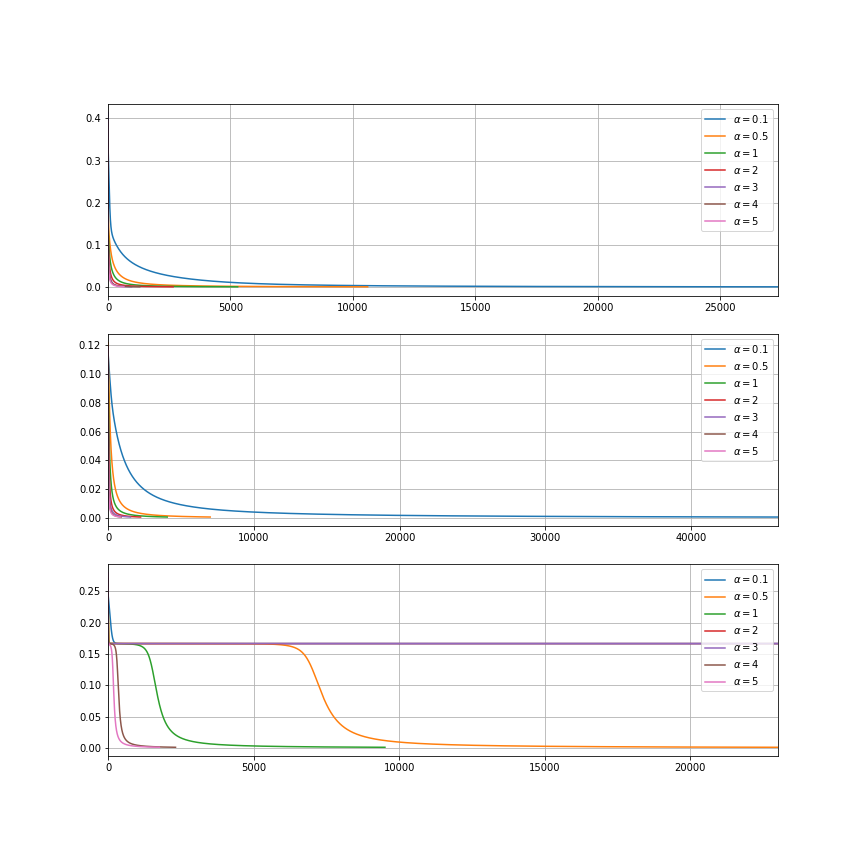
\includegraphics[width=17cm,height=20cm]{Training Batch 4 Orden 3.png}
    \caption{Entrenamiento de las redes con batch 4 (De arriba a abajo: And,Or,Xor)}
    \label{fig:TrainBatch4_Order3}
\end{figure}
\begin{figure}[H]
    \centering
    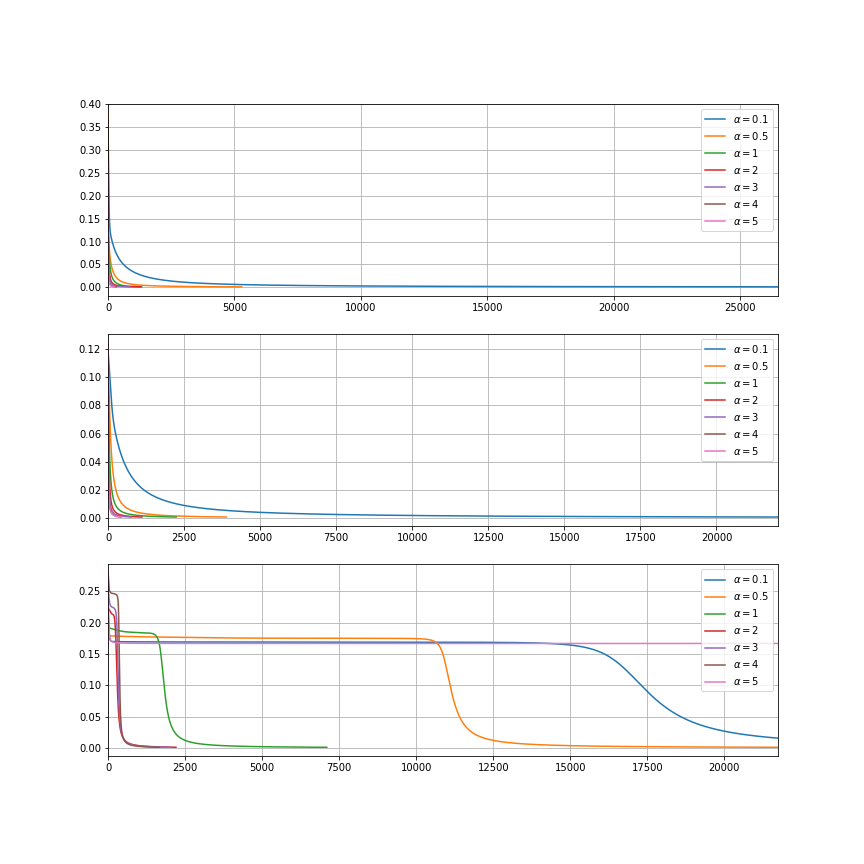
\includegraphics[width=17cm,height=20cm]{Training Batch 2 Orden 3.png}
    \caption{Entrenamiento de las redes con batch 2 (De arriba a abajo: And,Or,Xor)}
    \label{fig:TrainBatch2_Order3}
\end{figure}

    %\section{Información preliminar.}

    %\section{Metodologías.}

    \section{Resultados}
    \begin{table}[H]
    \centering
    \resizebox{17cm}{2cm}{
        \begin{tabular}{|l|l|l|l|l|l|l|}
            \hline
            \multicolumn{7}{|c|}{Letras: A,B,C,D,E}                                                                                                                                                                                                                                                                                                                                                                                                                                                                                                                                                                                                                                                                                      \\ \hline
            \multicolumn{7}{|c|}{Vigilancia}                                                                                                                                                                                                                                                                                                                                                                                                                                                                                                                                                                                                                                                                                             \\ \hline
            $\rho$                                                     & $0.1$                                                                                                    & $0.3$                                                                                                    & $0.5$                                                                                                    & $0.7$                                                                                                    & $0.9$                                                                                                    & $0.999$                                                                                                  \\ \hline
            \begin{tabular}[c]{@{}l@{}}Orden:\\ A,B,C,D,E\end{tabular} & \begin{tabular}[c]{@{}l@{}}Aprendizaje en 5 epocas\\ y genera 2 clusters\\ de clasificación\end{tabular} & \begin{tabular}[c]{@{}l@{}}Aprendizaje en 5 epocas\\ y genera 2 clusters\\ de clasificación\end{tabular} & \begin{tabular}[c]{@{}l@{}}Aprendizaje en 5 epocas\\ y genera 2 clusters\\ de clasificación\end{tabular} & \begin{tabular}[c]{@{}l@{}}Aprendizaje en 5 epocas\\ y genera 3 clusters\\ de clasificación\end{tabular} & \begin{tabular}[c]{@{}l@{}}Aprendizaje en 5 epocas\\ y genera 4 clusters\\ de clasificación\end{tabular} & \begin{tabular}[c]{@{}l@{}}Aprendizaje en 5 epocas\\ y genera 4 clusters\\ de clasificación\end{tabular} \\ \hline
            \begin{tabular}[c]{@{}l@{}}Orden:\\ C,E,A,B,D\end{tabular} & \begin{tabular}[c]{@{}l@{}}Aprendizaje en 5 epocas\\ y genera 2 clusters\\ de clasificación\end{tabular} & \begin{tabular}[c]{@{}l@{}}Aprendizaje en 5 epocas\\ y genera 2 clusters\\ de clasificación\end{tabular} & \begin{tabular}[c]{@{}l@{}}Aprendizaje en 5 epocas\\ y genera 2 clusters\\ de clasificación\end{tabular} & \begin{tabular}[c]{@{}l@{}}Aprendizaje en 5 epocas\\ y genera 3 clusters\\ de clasificación\end{tabular} & \begin{tabular}[c]{@{}l@{}}Aprendizaje en 5 epocas\\ y genera 4 clusters\\ de clasificación\end{tabular} & \begin{tabular}[c]{@{}l@{}}Aprendizaje en 5 epocas\\ y genera 5 clusters\\ de clasificación\end{tabular} \\ \hline
        \end{tabular}
    }
\end{table}

\begin{table}[H]
    \centering
    \resizebox{17cm}{!}{
        \begin{tabular}{|l|l|l|l|l|l|l|}
            \hline
            \multicolumn{7}{|c|}{Números: 0,1,2,3,4,5,6,7,8,9,}                                                                                                                                                                                                                                                                                                                                                                                                                                                                                                                                                                                                                                                                                                                             \\ \hline
            \multicolumn{7}{|c|}{Vigilancia}                                                                                                                                                                                                                                                                                                                                                                                                                                                                                                                                                                                                                                                                                                                                                \\ \hline
            $\rho$                                                                    & $0.1$                                                                                                          & $0.3$                                                                                                          & $0.5$                                                                                                          & $0.7$                                                                                                          & $0.9$                                                                                                          & $0.999$                                                                                                        \\ \hline
            \begin{tabular}[c]{@{}l@{}}Orden:\\ 1,2,3,4,5\\ 6,7,8,9,0\end{tabular}    & \begin{tabular}[c]{@{}l@{}}Aprendizaje en\\ 10 epocas\\ y genera \\ 4 clusters\\ de clasificación\end{tabular} & \begin{tabular}[c]{@{}l@{}}Aprendizaje en\\ 10 epocas\\ y genera\\ 4 clusters\\ de clasificación\end{tabular}  & \begin{tabular}[c]{@{}l@{}}Aprendizaje en\\ 10 epocas\\ y genera\\ 5 clusters\\ de clasificación\end{tabular}  & \begin{tabular}[c]{@{}l@{}}Aprendizaje en\\ 10 epocas\\ y genera\\ 6 clusters\\ de clasificación\end{tabular}  & \begin{tabular}[c]{@{}l@{}}Aprendizaje en\\ 10 epocas\\ y genera\\ 8 clusters\\ de clasificación\end{tabular}  & \begin{tabular}[c]{@{}l@{}}Aprendizaje en\\ 10 epocas\\ y genera\\ 10 clusters\\ de clasificación\end{tabular} \\ \hline
            \begin{tabular}[c]{@{}l@{}}Orden:\\ 1,6,0,2,3,5,\\ 8,7,4,9,1\end{tabular} & \begin{tabular}[c]{@{}l@{}}Aprendizaje en\\ 11 epocas\\ y genera \\ 4 clusters\\ de clasificación\end{tabular} & \begin{tabular}[c]{@{}l@{}}Aprendizaje en\\ 11 epocas\\ y genera \\ 4 clusters\\ de clasificación\end{tabular} & \begin{tabular}[c]{@{}l@{}}Aprendizaje en\\ 11 epocas\\ y genera \\ 4 clusters\\ de clasificación\end{tabular} & \begin{tabular}[c]{@{}l@{}}Aprendizaje en\\ 11 epocas\\ y genera \\ 6 clusters\\ de clasificación\end{tabular} & \begin{tabular}[c]{@{}l@{}}Aprendizaje en\\ 11 epocas\\ y genera \\ 9 clusters\\ de clasificación\end{tabular} & \begin{tabular}[c]{@{}l@{}}Aprendizaje en\\ 11 epocas\\ y genera \\ 9 clusters\\ de clasificación\end{tabular} \\ \hline
        \end{tabular}
    }
\end{table}

Se observa que para los patrones de las letras, la red si es capaz de lograr un aprendizaje que pueda
calsificar todas las letras de entrada \textbf{a,b,c,d} y \textbf{e} en un solo caso, en el de $\rho=0.999$,
y con el orden 2 de entrenamientos de la red.
Para el caso del entrenamiento de la red para la clasificación visual de los números, la red es capaz
de diferenciar todos los números solo si el orden de entrenamiento es el orden 1 y además de que el
parámetros $\rho=0.999$.
Por lo que se concluye que, para esta tarea de clasificación, utilizar un valor de $\rho$ más grande, permite
una mejor discerción de los datos de entrenamiento ya que se detectan diferencias ``más finas'' en el
conjunto de entrenamiento, mientras que, utilizar un valor de $\rho$ más pequeño, evita que la red pueda
detectar pequeñas diferencias entre un elemento del conjunto de entrenamiento y otro, por lo que su entrenamiento
resulta en la generación de menos ``clusters'' para la clasificación de la tareas.

    %\section{Conclusiones}
    %Se observó que los mapas mentales pueden ser utilizados con diversos fines y permiten tener una perspectiva
más clara y global acerca de un tema en especifico, ademas de que la misma naturalez de su estructura permite
añadir o quitar información de manera sencilla sin afectar todo lo demás. Se concluye además que, el uso
del mapa mental para esta actividad en especifico (Determinar en que invertimos nuestro tiempo) nos permite
tener noción de cuales son las cosas o actividades que más consumen de nuestro tiempo y en base a esta
información poder tomar mejores decisiones respecto a la organización del tiempo con el fin de lograr
nuestros objetivos.

    %%%%%%% Bibliografía %%%%%%%%
    %\addcontentsline{toc}{section}{Referencias}
    %\nocite{}
    %\bibliographystyle{IEEEtran}
    %\bibliography{bibliografia}

    %%%%%%% Apendice %%%%%%%%
    %\appendix
    %\clearpage
    %\addappheadtotoc
    %\appendixpage

\end{document}